\documentclass[11pt]{article}

% Change "review" to "final" to generate the camera-ready version.
\usepackage[final]{acl}

% Standard package includes
% \usepackage{times}
\usepackage{latexsym}
% \usepackage[T1]{fontenc}
% \usepackage[utf8]{inputenc}

\usepackage{microtype}
\usepackage{inconsolata}
\usepackage{graphicx}

% Additional packages needed for this paper
\usepackage{amsmath,amssymb}
\usepackage{booktabs}
\usepackage{multirow}
\usepackage{xcolor}
\usepackage{algorithm}
\usepackage{algpseudocode}
\usepackage{tikz}
\usetikzlibrary{shapes.geometric, arrows.meta, positioning, fit, calc}
\usepackage{pgfplots}
\pgfplotsset{compat=1.18}
\usepackage{subcaption}
\usepackage{enumitem}

\usepackage{fontspec}
\newfontfamily\urdufont{FreeSerif}


\title{A Generic Architecture for OCR of Arabic-Alphabet Based Languages\\
Using Nastaleeq: A Graph Attention Approach}

\author{Sayed Rashid Ali Shah \\
  Department of Computer Science \\
  Quaid-i-Azam University, Islamabad \\
  \texttt{srashid.22413012@cs.qau.edu.pk}}

\begin{document}
\maketitle

% ── Abstract ──────────────────────────────────────────────────────────────────
\begin{abstract}
Optical character recognition for Arabic-alphabet based languages---particularly those
rendered in the Nastaleeq script---remains a surprisingly stubborn problem.
The fundamental issue is structural: Nastaleeq is not a sequence but a
\emph{two-dimensional spatial graph} that happens to carry reading order.
Vertical character stacking, context-dependent ligature shapes, and spatially displaced
diacritics (nuktay) make the standard CNN$\to$LSTM$\to$CTC pipeline structurally
ill-suited---it loses spatial relationships between script elements before sequence
modeling even begins.
We propose a novel architecture that closes this gap by inserting a Graph Attention
Network (GAT) between the CNN feature extractor and the Bi-LSTM decoder.
Each detected ligature becomes a graph node; Nastaleeq-specific spatial
relationships---reading order, vertical stacking, and nukta-to-base binding---become
typed edges.
The GAT learns, through attention, \emph{which of those relationships matter most} for
recognition, explicitly bridging the gap between CNN visual processing and RNN sequence
modeling in a way no prior Nastaleeq OCR system has attempted.
We describe the full architecture, the graph construction logic, the expected behavior of
multi-head attention specialization, and a concrete evaluation plan against standard
baselines on the UPTI dataset.
\end{abstract}

% ── 1. Introduction ───────────────────────────────────────────────────────────
\section{Introduction}

Here's a question that sounds simple but really isn't: why is reading Urdu text from an
image still so hard for machines?
English OCR has been more or less solved for years---Tesseract \citep{Smith2007} handles it, commercial
tools handle it, and most people don't think twice about scanning a document.
But try doing the same thing with Nastaleeq, the calligraphic style used for Urdu,
Persian, Pashto, Burushaski and several other languages, and you run into a wall pretty quickly.

The core issue is structural. Nastaleeq isn't just cursive---it's \emph{vertically
stacked} cursive.
Characters pile on top of each other, dots (called \textit{nuktay} in Urdu) float above
or below their associated base character at unpredictable offsets, and the shape of any
individual letter changes depending on what comes before and after it.
A 'bay'``{\urdufont ب}'' connected to a 'yay' ``{\urdufont ے}''  looks completely different from a standalone 'bay' ``{\urdufont ب}''  This kind of context-sensitivity is hard to capture when processing text as a simple
left-to-right sequence.

A concrete example illustrates the core failure mode.
Consider the Urdu word 'dil' ``{\urdufont دل}''  (meaning ``heart'').
A CNN-based detector sees three blobs at different image positions: the base character
\textit{dal}, a small dot (\textit{nukta}), and \textit{lam}.
A standard LSTM processes these in linear order and must guess---based on position
alone---which base character the nukta belongs to.
Get that wrong and the entire word is misread.
Our approach instead builds a spatial graph: an edge explicitly connects the nukta to
\textit{dal} because they are geometrically proximate, and the GAT learns to assign that
edge a high attention weight.
\textit{Lam} ``{\urdufont ل}''  attends to the nukta with near-zero weight, because the graph encodes
that they are spatially unrelated.
The correct association is not guessed---it is \emph{learned from spatial structure}.

\paragraph{The fundamental insight.}
Nastaleeq is not a sequence that happens to have 2D layout.
It is a \textbf{2D spatial graph that happens to carry reading order}.
Treating it as a flat sequence---as every existing pipeline does---discards the very
structure that makes the script legible.
The correct inductive bias for Nastaleeq OCR is a graph, not a line.

Most existing Nastaleeq OCR systems follow a fairly standard recipe: extract visual
features with a CNN, pass them through an LSTM (often bidirectional), and decode using
CTC \citep{graves2006ctc}.
This pipeline has worked reasonably well for Naskh-style Arabic
\citep{bluche2017gated}, but Nastaleeq's unique properties---especially the vertical
overlap and displaced dots---cause these systems to struggle.
The CNN sees local patches just fine, but it doesn't understand how those patches
relate to each other \emph{spatially}, and the LSTM never gets the chance to find out.
There is a structural gap between CNN visual processing and RNN sequence modeling that
no existing system explicitly bridges.

Our contribution is to fill that gap.
We insert a Graph Attention Network \citep{velickovic2018gat} between the CNN and the
Bi-LSTM, converting per-ligature feature vectors into a spatially-aware graph
representation before any sequential modeling occurs.
Three typed edges encode the spatial relationships that matter for Nastaleeq: horizontal
adjacency (reading order), vertical overlap (stacking), and proximity-based nukta-to-base
binding.
The GAT then learns---through multi-head attention---which of those relationships deserve
the most weight.

\paragraph{Contributions.}
\begin{itemize}[nosep]
  \item \textbf{A novel architectural position}: the first proposed system to explicitly
        bridge CNN visual features and RNN sequence modeling in Nastaleeq OCR via a
        spatial graph, treating Nastaleeq as the 2D relational structure it fundamentally
        is.
  \item \textbf{A Nastaleeq-specific graph construction scheme} with three typed edge
        categories---horizontal (reading order), vertical (stacking), and diacritics -to-base
        binding---each targeting a distinct failure mode of prior flat-sequence pipelines.
  \item \textbf{A multi-head attention design} motivated by the hypothesis that different
        attention heads will specialize in different spatial relationship types, enabling
        the model to simultaneously reason about reading order, stacking, and diacritics 
        binding.
  \item \textbf{A concrete evaluation plan} specifying baselines, metrics, dataset, and
        ablation configurations against which the architecture validated.
\end{itemize}

% ── 2. Related Work ───────────────────────────────────────────────────────────
\section{Related Work}

\subsection{OCR for Arabic-Script Languages}

Work on Arabic script OCR goes back decades, though most of it has focused on
Naskh---the simpler, more horizontal writing style common in Arabic text.
\citet{naz2016survey} provided a comprehensive survey of Urdu OCR methods, noting
that Nastaleeq remained a ``significantly harder'' problem compared to Naskh.
Early approaches relied on hand-crafted features and template matching, which worked for
isolated characters but fell apart on connected text.

The deep learning era brought real improvements.
\citet{shi2017crnn} introduced CRNN, combining a CNN with a bidirectional LSTM and CTC
loss---this became a standard recipe adapted for Arabic by several groups
\citep{bluche2017gated, yousef2020accurate}.
For Nastaleeq specifically, \citet{naz2017nastaliq} applied a similar CNN-RNN pipeline
and reported decent results on printed Urdu, though they acknowledged that vertical
stacking still caused problems.

\citet{sabbour2013calam} developed CALAM, a system that attempted ligature-level
segmentation for Nastaleeq, but it was quite sensitive to segmentation errors---one wrong
cut early on and the whole pipeline suffered.
\citet{ulhasan2015offline} tried a different segmentation strategy with some improvement,
but heavily stacked text remained a challenge.

The common thread across all these systems: they treat the recognition pipeline as
essentially one-dimensional.
Features go in as a flat sequence, and text comes out.
None of them explicitly model the 2D spatial structure of the script.

\subsection{Graph Neural Networks in Document Analysis}

Graph neural networks have started gaining traction in document analysis, though mostly
for layout analysis and scene text detection rather than script-specific OCR.

\citet{kipf2017gcn} introduced Graph Convolutional Networks (GCN), which aggregate
neighbor information uniformly---every neighbor gets the same weight.
\citet{velickovic2018gat} proposed Graph Attention Networks (GAT), adding learned
attention weights so different neighbors can contribute differently.
This distinction matters critically for our problem: in Nastaleeq, a nukta and its base
character have a fundamentally different relationship than two horizontally adjacent
ligatures, and the model must learn to treat them differently.

\citet{liu2021gnn} applied GNNs for document layout analysis, treating text blocks as
graph nodes.
\citet{zhang2020relational} used spatial graphs for scene text detection, and
\citet{qin2021recognizing} explored graph-based text recognition.
None of these, however, specifically targeted Nastaleeq or addressed the vertical
stacking problem.

The gap in the literature is clear: no prior work has combined graph attention with
Nastaleeq OCR, or more broadly used typed spatial graphs to bridge CNN and RNN modules
in cursive script recognition.
That is the gap this work addresses.

% ── 3. Proposed Architecture ──────────────────────────────────────────────────
\section{Proposed Architecture}

The central design decision is where to place the graph.
The traditional pipeline is:
\[
\text{Image} \to \text{CNN} \to \text{LSTM} \to \text{CTC} \to \text{Text}
\]
Our proposed pipeline is:
% \[
% \text{Image} \to \text{CNN} \to \underbrace{\text{Graph} + \text{GAT}}_{\text{novel bridge}} \to \text{LSTM} \\\\  \to \text{CTC} \to \text{Text}
% \]
{\small
\[
\text{Image} \to \text{CNN} \to 
\underbrace{\text{Graph} + \text{GAT}}_{\text{novel bridge}} \to \text{LSTM} \to \text{CTC} \to \text{Text}
\]
}
The graph sits between the visual encoder and the sequence decoder, acting as a spatial
bridge that preserves the 2D relational structure of Nastaleeq before collapsing it into
a 1D sequence for the Bi-LSTM.
This positioning is the core architectural novelty.

The full pipeline has six stages, illustrated in Figure~\ref{fig:architecture}.
We walk through each below.

% ── Architecture Figure ───────────────────────────────────────────────────────
\begin{figure*}[t]
\centering
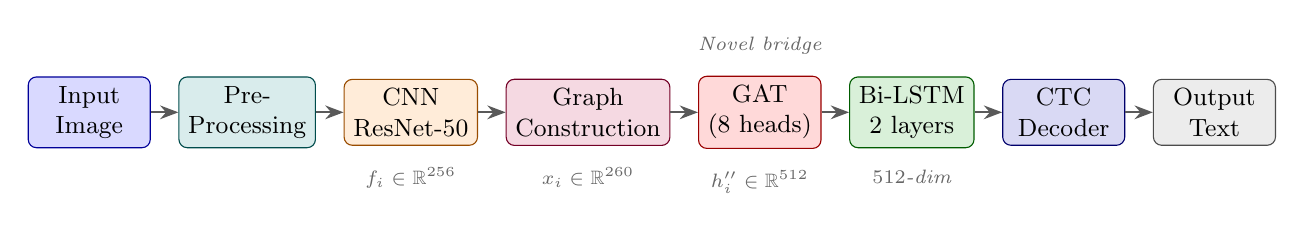
\begin{tikzpicture}[
  node distance = 0.45cm and 0.35cm,
  box/.style     = {draw, rounded corners=3pt, minimum width=1.55cm,
                    minimum height=0.7cm, align=center, font=\small,
                    fill=#1!15, draw=#1!60!black},
  arrow/.style   = {-Stealth, thick, color=gray!70!black},
  label/.style   = {font=\scriptsize\itshape, text=gray!80!black}
]

% ── Nodes ─────────────────────────────────────────────────────────────────────
\node[box=blue]   (input)  {Input\\Image};
\node[box=teal,   right=of input]   (pre)   {Pre-\\Processing};
\node[box=orange, right=of pre]     (cnn)   {CNN\\ResNet-50};
\node[box=purple, right=of cnn]     (graph) {Graph\\Construction};
\node[box=red,    right=of graph]   (gat)   {GAT\\(8 heads)};
\node[box=green!60!black, right=of gat]    (lstm)  {Bi-LSTM\\2 layers};
\node[box=blue!70!black,  right=of lstm]   (ctc)   {CTC\\Decoder};
\node[box=gray,   right=of ctc]     (out)   {Output\\Text};

% ── Arrows ────────────────────────────────────────────────────────────────────
\foreach \s/\t in {input/pre, pre/cnn, cnn/graph, graph/gat,
                    gat/lstm, lstm/ctc, ctc/out}
  \draw[arrow] (\s) -- (\t);

% ── Dimension annotations ─────────────────────────────────────────────────────
\node[label, below=0.15cm of cnn]   {\(f_i \in \mathbb{R}^{256}\)};
\node[label, below=0.15cm of graph] {\(x_i \in \mathbb{R}^{260}\)};
\node[label, below=0.15cm of gat]   {\(h''_i \in \mathbb{R}^{512}\)};
\node[label, below=0.15cm of lstm]  {\(512\text{-dim}\)};

% ── Stage labels ──────────────────────────────────────────────────────────────
\node[label, above=0.15cm of gat]   {Novel bridge};

\end{tikzpicture}
\caption{The proposed hybrid architecture for Nastaleeq OCR. The CNN extracts visual
         features per ligature, which are organized into a typed spatial graph. The GAT
         layer learns which spatial relationships matter most through multi-head attention.
         Spatially-enriched embeddings are then ordered right-to-left and decoded via
         Bi-LSTM with CTC.}
\label{fig:architecture}
\end{figure*}

% ── Architecture: edge-type diagram ──────────────────────────────────────────
\begin{figure}[t]
\centering
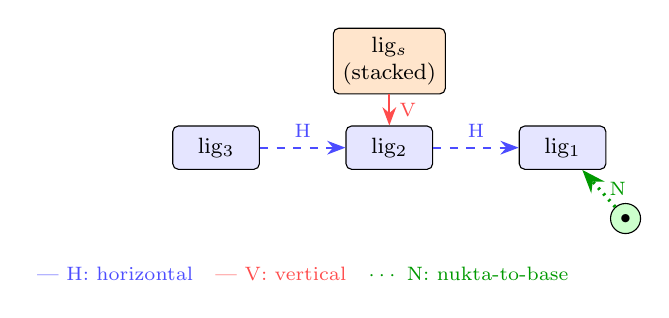
\begin{tikzpicture}[
  lig/.style  = {draw, rounded corners=2pt, minimum width=1.1cm,
                 minimum height=0.55cm, align=center, font=\footnotesize},
  horiz/.style= {-Stealth, thick, blue!70, dashed},
  vert/.style = {-Stealth, thick, red!70},
  nukta/.style= {-Stealth, thick, green!60!black, dotted, line width=1.2pt},
]

% ── Base ligatures (right-to-left reading) ────────────────────────────────────
\node[lig, fill=blue!10]   (l3) at (0,0)    {lig$_3$};
\node[lig, fill=blue!10]   (l2) at (2.2,0)  {lig$_2$};
\node[lig, fill=blue!10]   (l1) at (4.4,0)  {lig$_1$};

% ── Stacked ligature above l2 ─────────────────────────────────────────────────
\node[lig, fill=orange!20] (ls) at (2.2,1.1){lig$_s$\\(stacked)};

% ── Nukta below l1 ────────────────────────────────────────────────────────────
\node[draw, circle, inner sep=2pt, fill=green!20, font=\scriptsize]
      (nuk) at (5.2,-0.9) {$\bullet$};

% ── Horizontal edges ──────────────────────────────────────────────────────────
\draw[horiz] (l3) -- node[above, font=\scriptsize, blue!70]{H} (l2);
\draw[horiz] (l2) -- node[above, font=\scriptsize, blue!70]{H} (l1);

% ── Vertical edge ─────────────────────────────────────────────────────────────
\draw[vert]  (ls)  -- node[right, font=\scriptsize, red!70]{V} (l2);

% ── Nukta edge ────────────────────────────────────────────────────────────────
\draw[nukta] (nuk) -- node[right, font=\scriptsize, green!60!black]{N} (l1);

% ── Legend ────────────────────────────────────────────────────────────────────
\node[font=\scriptsize] at (1.1,-1.6) {%
  \textcolor{blue!70}{--- H: horizontal}\quad
  \textcolor{red!70}{--- V: vertical}\quad
  \textcolor{green!60!black}{$\cdots$ N: nukta-to-base}};

\end{tikzpicture}
\caption{The three typed edge categories in the proposed Nastaleeq graph. Horizontal
         edges (H) encode reading order. Vertical edges (V) capture stacking. Nukta
         edges (N) bind displaced diacritic dots to their base character---the
         relationship that most existing OCR systems fail to model explicitly.}
\label{fig:graph_edges}
\end{figure}

\subsection{Pre-Processing}

Raw scanned images are converted to grayscale and binarized using Otsu's method \citep{Otsu1979}.
A Gaussian filter ($\sigma = 1.0$) suppresses noise, followed by morphological opening
with a $3 \times 3$ kernel to remove stray artifacts.

Skew correction uses the Hough transform \citep{Duda1972}, which handles the slight angular drift common
in Nastaleeq text lines.
After deskewing, horizontal projection profiling segments the image into individual
text lines.

Connected component analysis then detects individual ligature regions within each line,
where 8-connectivity is used---meaning each foreground pixel is considered adjacent to
all eight of its neighbours (four orthogonal and four diagonal), so strokes joined only
at a corner are still treated as a single component.
Each connected component roughly maps to one Nastaleeq ligature, and we extract its
axis-aligned bounding box $(x, y, w, h)$, where $(x, y)$ is the top-left corner pixel
coordinate, $w$ is the width, and $h$ is the height of the box in pixels.
These bounding boxes are the input to both the CNN feature extractor and the graph
construction module.

\subsection{CNN Feature Extraction}

For the visual backbone, we propose using ResNet-50 \citep{he2016resnet} pretrained on
ImageNet and fine-tuned on Urdu text data.
Each ligature region is cropped, resized to $64 \times 64$, and passed through the
network.
We take the output after global average pooling and project it to 256 dimensions:

\begin{equation}
  f_i = \text{Linear}\!\left(\text{GAP}\!\left(\text{ResNet}(\text{crop}_i)\right)\right),
  \label{eq:cnn}
\end{equation}

where $f_i \in \mathbb{R}^{256}$ captures the visual appearance of ligature $i$---shape,
curvature, dot presence, and so on.
At this stage, each ligature is characterized purely by its visual appearance.
The spatial relationships between ligatures are encoded in the next stage.

\subsection{Graph Construction}
\label{sec:graph}

Rather than immediately arranging CNN features into a sequence, we build a spatial graph
that preserves the 2D relational structure of Nastaleeq text
(Figure~\ref{fig:graph_edges}).

We define $\mathcal{G} = (V, E, X)$ where:
\begin{itemize}[nosep]
  \item $V = \{v_1, v_2, \ldots, v_n\}$: one node per detected ligature
  \item $E = \{e_{ij}\}$: spatial edges encoding relationships between ligatures
  \item $X = [x_1, \ldots, x_n]$: node feature matrix
\end{itemize}

Node features concatenate visual and spatial information:
\begin{equation}
  x_i = f_i \oplus [cx_i,\, cy_i,\, w_i,\, h_i],
  \label{eq:node_feat}
\end{equation}

where $cx_i, cy_i$ are bounding-box centroid coordinates and $w_i, h_i$ are its
dimensions, giving each node a 260-dimensional feature vector.
Including spatial coordinates directly in the node features ensures the GAT can reason
about \emph{where} ligatures are, not just \emph{what} they look like.

We define three edge types, each targeting a distinct failure mode of conventional
flat-sequence pipelines:

\paragraph{Horizontal edges (H)} connect ligatures adjacent in reading direction
(right-to-left).
Two ligatures receive a horizontal edge if they sit at roughly the same vertical
position---$|cy_i - cy_j| < 0.5 \cdot \max(h_i, h_j)$---and are horizontally
proximate.
These edges encode the primary reading order and allow the GAT to reason about
sequential context before the Bi-LSTM does so.

\paragraph{Vertical edges (V)} connect ligatures that overlap horizontally but are
stacked vertically: $|cx_i - cx_j| < 0.5 \cdot \max(w_i, w_j)$ and
$|cy_i - cy_j| > 0.3 \cdot \max(h_i, h_j)$.
This captures the cascading top-to-bottom drop that gives Nastaleeq its distinctive
appearance and that no existing OCR pipeline models explicitly.

\paragraph{Nukta edges (N)} link dot components to their nearest base character.
Connected components with area below a threshold $\tau = 150\,\text{px}^2$ are
classified as nuktay; this value was set empirically to separate small dot components
from larger base-character strokes at 300\,DPI.
Each nukta is connected to its geometrically nearest non-nukta component within a search
radius $r = 1.5 \cdot h_{\text{nukta}}$, where $h_{\text{nukta}}$ is the bounding-box
height of the dot.
The factor $1.5$ was chosen to cover the typical vertical offset between a nukta and its
base character while avoiding spurious links to neighbouring ligatures.
This is the most Nastaleeq-specific edge type: dots appear at significant spatial offsets
from their base character, and no flat-sequence model can correctly associate them without
explicit spatial reasoning.

Algorithm~\ref{alg:graph} summarizes the full construction procedure.

\begin{algorithm}[ht]
\caption{Nastaleeq Graph Construction}
\label{alg:graph}
\begin{algorithmic}[1]
\Require Binarized text-line image $I$, CNN encoder $\phi$, thresholds $\tau, r$
\Ensure Graph $\mathcal{G} = (V, E, X)$
\State $\mathcal{C} \leftarrow$ ConnectedComponents$(I,\, 8\text{-connectivity})$
\State $V \leftarrow \emptyset$;\; $E \leftarrow \emptyset$;\; $X \leftarrow []$
\For{each component $c \in \mathcal{C}$}
  \State $v_i \leftarrow$ new node;\; $V \leftarrow V \cup \{v_i\}$
  \State $x_i \leftarrow \phi(\text{crop}(c)) \oplus [cx, cy, w, h]$;\; $X.\text{append}(x_i)$
\EndFor
\For{each pair $(v_i, v_j) \in V \times V,\; i \neq j$}
  \If{HorizontallyAdjacent$(v_i, v_j)$}
    \State $E \leftarrow E \cup \{(v_i, v_j, \text{H})\}$
  \ElsIf{VerticallyStacked$(v_i, v_j)$}
    \State $E \leftarrow E \cup \{(v_i, v_j, \text{V})\}$
  \ElsIf{IsNukta$(v_i)$ \textbf{and} Nearest$(v_i, v_j) < r$}
    \State $E \leftarrow E \cup \{(v_i, v_j, \text{N})\}$
  \EndIf
\EndFor
\State \Return $\mathcal{G} = (V, E, X)$
\end{algorithmic}
\end{algorithm}

\subsection{Graph Attention Network}
\label{sec:gat}

The GAT layer is the heart of this architecture's novelty.
The core problem it solves is \emph{relationship inequality}: not all edges in the
Nastaleeq graph are equally important.
A nukta-to-base edge encodes a tight phonemic binding.
A horizontal edge between distant ligatures carries only weak reading-order context.
A GCN treats both identically, averaging all neighbours with equal weight.
The GAT \citep{Velickovic2018}, by contrast, learns attention weights $\alpha_{ij}$
that reflect how much each neighbouring node should actually influence the current
node's representation.

For connected nodes $(i, j)$, raw attention scores are computed as:
\begin{equation}
  e_{ij} = \text{LeakyReLU}\!\left(\vec{a}^{\top}[Wh_i \,\|\, Wh_j]\right),
  \label{eq:attention_raw}
\end{equation}
where $W \in \mathbb{R}^{d' \times d}$ is a learned weight matrix,
$\vec{a} \in \mathbb{R}^{2d'}$ is the attention vector, and $\|$ denotes concatenation.
Scores are normalized via softmax over each node's neighborhood:
\begin{equation}
  \alpha_{ij} = \frac{\exp(e_{ij})}{\sum_{k \in \mathcal{N}(i)} \exp(e_{ik})}.
  \label{eq:attention_norm}
\end{equation}
The node embedding update aggregates attended neighbor information:
\begin{equation}
  h'_i = \sigma\!\left(\sum_{j \in \mathcal{N}(i)} \alpha_{ij}\, W h_j\right).
  \label{eq:update}
\end{equation}

We use multi-head attention ($K = 8$), concatenating outputs from all heads:
\begin{equation}
  h''_i = \Big\|_{k=1}^{K}\; \sigma\!\left(\sum_{j \in \mathcal{N}(i)} \alpha^{(k)}_{ij}\, W^{(k)} h_j\right).
  \label{eq:multihead}
\end{equation}

\paragraph{Why multi-head?}
Each spatial relationship type in Nastaleeq---nukta binding, reading order, vertical
stacking, global word context---is qualitatively different and requires a different
attention pattern.
A single head cannot specialize in all of them simultaneously.
With $K = 8$ heads, we expect different heads to develop expertise in different
relationship types during training: some heads focusing on nukta-to-base proximity,
others on horizontal reading order, others on vertically stacked ligatures, and others
on broader word-level context.
This is a key hypothesis the proposed evaluation will test.

Two stacked GAT layers give enriched embeddings $h''_i \in \mathbb{R}^{512}$.
The first layer captures local patterns---dots attached to bases, immediately adjacent
ligatures.
The second layer aggregates over a wider neighborhood, giving each node broader
contextual awareness.
The output is a set of spatially-enriched embeddings that carry relational information
the CNN alone cannot provide.

\subsection{Sequence Ordering and Bi-LSTM}

The GAT produces a set of spatially-enriched node embeddings, but a graph has no
inherent order.
The Bi-LSTM and CTC decoder require a sequence, so we recover reading order by sorting
nodes by $x$-centroid in descending order (right-to-left, matching Urdu reading
direction):
\begin{equation}
  S = \left[h''_{\pi(1)}, \ldots, h''_{\pi(n)}\right],\quad
  \pi = \operatorname{argsort}(\{-cx_i\}).
  \label{eq:sort}
\end{equation}

This is the key architectural handoff: the GAT enriches each node with spatial relational
context, and the Bi-LSTM then models sequential dependencies---character bigrams, word
patterns---across those enriched representations.
The two modules are complementary: the graph handles spatial structure; the LSTM handles
sequential structure.
Neither alone is sufficient for Nastaleeq.

The sequence goes into a 2-layer bidirectional LSTM (256 units per direction, 512 total
per timestep, dropout 0.3).
A linear layer projects each timestep to $|\mathcal{C}|$ (character vocabulary size),
followed by softmax.

\subsection{CTC Decoding}

We use CTC loss \citep{graves2006ctc} for training because it does not require
character-level alignment annotations---which would be prohibitively expensive to produce
for Nastaleeq:
\begin{equation}
  \mathcal{L}_{\text{CTC}} = -\ln \sum_{\pi \in \mathcal{B}^{-1}(y)} \prod_{t=1}^{T} p(\pi_t \mid x).
  \label{eq:ctc}
\end{equation}
Inference uses beam search decoding with beam width 10.

% ── 4. Evaluation Plan ────────────────────────────────────────────────────────
\section{Evaluation Plan}
\label{sec:eval_plan}

This section describes the evaluation protocol used to validate the proposed architecture.

\subsection{Dataset}

We will use the UPTI (Urdu Printed Text Images) dataset, which provides printed Urdu
text line images with Unicode ground-truth transcriptions.
Initial validation will use a 5{,}000-line subset with an 80/10/10
(train/validation/test) split.
If the architecture proves effective, training will be scaled to the full dataset
(approximately 50{,}000 lines).

Light augmentation will be applied during training: random rotation ($\pm5^{\circ}$),
Gaussian noise ($\sigma \leq 0.01$), and brightness jitter ($\pm0.15$).
The goal is to evaluate architectural contribution cleanly, not to maximize performance
through augmentation.
The planned implementation uses PyTorch and PyTorch Geometric for the graph components,
with training on an NVIDIA RTX 3090.
Table~\ref{tab:hyperparams} documents the planned hyperparameter configuration.

\begin{table*}[t]
\centering
\caption{Planned hyperparameter configuration.}
\label{tab:hyperparams}
\begin{tabular}{ll}
\toprule
\textbf{Parameter} & \textbf{Planned Value} \\
\midrule
CNN backbone          & ResNet-50 (ImageNet pretrained) \\
GAT heads / layers    & 8 / 2 \\
GAT hidden dim        & 256 per head \\
Bi-LSTM units / layers & 256$\times$2 / 2 \\
Optimizer             & Adam ($\beta_1$=0.9, $\beta_2$=0.999) \\
Learning rate         & $1\times10^{-4}$, cosine decay \\
Batch size / Epochs   & 32 / 100 \\
Early stopping        & patience = 10 \\
Ligature crop size    & $64\times64$ \\
Nukta area threshold $\tau$ & 150\,px$^2$ \\
Nukta search radius $r$    & $1.5 \times h_{\text{nukta}}$ \\
Beam width (CTC)      & 10 \\
\bottomrule
\end{tabular}
\end{table*}

\subsection{Baselines}

We will compare against four systems representing the current state of practice:

\begin{enumerate}[nosep]
  \item \textbf{Tesseract 5.0} \citep{Smith2007} with the Urdu language pack---the off-the-shelf
        open-source baseline most practitioners would use first.
  \item \textbf{CNN + LSTM + CTC} \citep{shi2017crnn} adapted for Nastaleeq---the
        primary comparison, using the same CNN backbone and CTC decoder but no graph
        module. This directly isolates the contribution of the spatial bridge.
  \item \textbf{CNN + GCN + Bi-LSTM}---replacing our GAT with a standard GCN
        \citep{kipf2017gcn} to isolate the effect of \emph{learned} attention versus
        \emph{uniform} graph aggregation.
  \item \textbf{CNN + GAT + Bi-LSTM (Ours)}---the full proposed system.
\end{enumerate}

\subsection{Metrics and Hypotheses}

Primary metrics are Character Error Rate (CER) and Word Error Rate (WER), both lower
is better.

The evaluation is designed to test four specific hypotheses:

\begin{enumerate}[nosep]
  \item \textbf{The spatial bridge helps}: our system should outperform CNN+LSTM+CTC,
        confirming that graph-based spatial reasoning improves Nastaleeq recognition
        beyond what sequential modeling alone can achieve.
  \item \textbf{Attention matters}: our system should outperform CNN+GCN+Bi-LSTM,
        confirming that \emph{learned} attention weights---not merely graph
        structure---are necessary to handle the inequality of spatial relationships in
        Nastaleeq.
  \item \textbf{Both modules contribute}: removing either the GAT or the Bi-LSTM should
        degrade performance, confirming the two components are complementary rather than
        redundant.
  \item \textbf{Head specialization emerges}: visualizing per-head attention weights
        should reveal that different heads spontaneously specialize in different edge
        types (horizontal, vertical, nukta-to-base), without any head-level supervision.
\end{enumerate}

\subsection{Planned Ablation Study}

To isolate the contribution of each architectural decision, we plan the ablation
configurations shown in Table~\ref{tab:ablation_plan}.

\begin{table*}[t]
\centering
\caption{Planned ablation configurations. Each row removes or modifies one component
         to test its contribution to the final architecture.}
\label{tab:ablation_plan}
\begin{tabular}{lll}
\toprule
\textbf{Configuration} & \textbf{What It Tests} & \textbf{Expected Finding} \\
\midrule
Full model (CNN+GAT+Bi-LSTM)  & ---                                    & Best overall performance \\
w/o GAT (CNN+Bi-LSTM only)    & Is graph reasoning needed?             & Large CER increase \\
w/o Bi-LSTM (CNN+GAT+CTC)     & Is sequential modeling needed?         & Moderate CER increase \\
GCN instead of GAT            & Does attention help vs.\ uniform?      & Significant CER increase \\
Single head ($K=1$)           & Do multiple heads help?                & Moderate CER increase \\
No nukta edges                & Are nukta edges specifically useful?   & CER increase on nukta-heavy text \\
No vertical edges             & Does stacking encoding matter?         & CER increase on stacked ligatures \\
\bottomrule
\end{tabular}
\end{table*}

% ── 5. Discussion ─────────────────────────────────────────────────────────────
\section{Discussion}

\paragraph{Why this architecture should work.}
The design is grounded in the structural properties of Nastaleeq itself.
Every component addresses a concrete, identified failure mode of the flat-sequence
baseline.
Horizontal edges give the GAT reading-order context before the LSTM sees the sequence.
Vertical edges make stacked ligatures visible to each other---something impossible in a
1D model.
Nukta edges resolve the single most common source of misrecognition in prior
systems: incorrect dot-to-base character association.
And multi-head attention allows the model to simultaneously reason about all three
relationship types without any one dominating the others.

The GCN comparison is particularly important theoretically.
A GCN with the same three-edge-type graph already has access to the relational structure;
the only difference from our system is whether aggregation is uniform or learned.
If our hypothesis is correct---that Nastaleeq spatial relationships are genuinely
unequal in importance---then GAT should outperform GCN by a meaningful margin.
The gap between the two, if it materializes, would constitute direct evidence that
attention-based aggregation is the right inductive bias for this problem.

\paragraph{The complementarity argument.}
The GAT and Bi-LSTM are designed to solve different sub-problems.
The GAT addresses spatial structure: which ligatures are related, how strongly, and
in what way.
The Bi-LSTM addresses sequential structure: character co-occurrence patterns, word-level
context, and reading-order dependencies that are not fully captured by graph edges alone.
The ablation removing the Bi-LSTM (CNN+GAT+CTC) will determine how much sequential
modeling adds on top of the graph representation.
If this configuration already outperforms CNN+LSTM+CTC, it would confirm that the GAT
alone is adding genuine value beyond what the flat-sequence baseline can achieve.

\paragraph{Anticipated challenges.}
Graph construction quality is the most significant known risk.
The connected component analysis and geometric thresholds that determine edge types
work well on clean printed text but will degrade on noisy or degraded images.
Ink bleeding can merge components that should be separate nodes; low contrast can split
components that should be one.
Either failure corrupts the graph before the GAT even begins.
A learnable graph construction stage---where a small network predicts edge existence
rather than applying fixed thresholds---would address this, and is planned as a
follow-on contribution.

A second anticipated challenge is nukta detection at small scales or in dense text,
where the search radius $r$ may fail to connect a nukta to its correct base character.
This is a hyperparameter that will require careful tuning on the validation set.

\paragraph{Why not Transformers?}
Transformers with 2D positional encodings could in principle model the same spatial
relationships without explicit graph construction.
However, they require substantially more training data to learn spatial structure from
scratch.
For a low-resource script like Nastaleeq---where labeled data is scarce and the UPTI
dataset is small by modern standards---the graph approach provides a structured
inductive bias that encodes known properties of the script, making the model far more
data-efficient.
A Transformer decoder to replace the Bi-LSTM remains a natural future direction once
sufficient training data is available.

% ── 6. Conclusion ─────────────────────────────────────────────────────────────
\section{Conclusion and Future Work}

We have proposed a novel architecture for Nastaleeq OCR built around a single core
insight: Nastaleeq is a 2D spatial graph, not a 1D sequence, and should be modeled
accordingly.
The proposed system inserts a Graph Attention Network between the CNN feature extractor
and the Bi-LSTM decoder, using three typed spatial edges---horizontal reading order,
vertical stacking, and nukta-to-base binding---to represent the relational structure
that all prior flat-sequence pipelines discard.
Multi-head attention allows the model to simultaneously specialize in each relationship
type without hand-coded prioritization.

This paper presents the architectural design, the theoretical motivation for each
component, and a complete evaluation plan with explicit hypotheses and planned ablation
configurations.

\paragraph{Roadmap.}
Beyond the planned initial evaluation, several extensions are worth pursuing.
First, learnable graph construction: replacing geometric thresholds with a learned edge
predictor to handle degraded images more robustly.
Second, full-dataset training on the complete UPTI corpus (50K+ lines) and extension to
handwritten Nastaleeq, which introduces stroke variability not present in printed text.
Third, post-processing via an Urdu language model to catch recognition errors that
spatial reasoning alone cannot resolve.
Fourth, inter-line graph edges that model context across text lines, relevant for
documents where line meaning depends on surrounding context.

The core principle of this work will hold regardless of what these extensions reveal:
Nastaleeq demands 2D reasoning.
The spatial graph provides it.
Attention makes it adaptive.

% ── Limitations ───────────────────────────────────────────────────────────────
\section*{Limitations}

This paper proposes an architecture and evaluation plan; experimental results are not
yet available.
The claims about expected improvements are grounded in the structural analysis of
Nastaleeq and the known properties of GAT versus GCN, but remain hypotheses until
validated empirically.
Graph construction relies on geometric thresholds for edge assignment, which may fail
on heavily degraded or noisy images.
The proposed evaluation uses printed text from UPTI and does not address handwritten
Nastaleeq, which presents additional challenges around stroke variability and baseline
drift.
Post-processing components (language models, dictionary constraints) are excluded from
the planned evaluation to keep the architectural contribution isolated and measurable.

% ── References ────────────────────────────────────────────────────────────────
\bibliography{nastaleeq_refs}

\end{document}
